\documentclass[a4paper]{article}
\usepackage[margin=1cm]{geometry}
\usepackage{graphicx}
\usepackage{siunitx}
\usepackage{tikz}
\usepackage{float}
\usepackage{multicol}   
\usetikzlibrary{shapes.geometric,calc}
\newcommand{\w}{4}
\begin{document}
\section{Highest degree of rotational symmetry?}
    \subsection{\ang{60} rotational summetry}
    \begin{multicols}{2}
        \subsubsection{Has reflection}
            \begin{figure}[H]
            \centering
            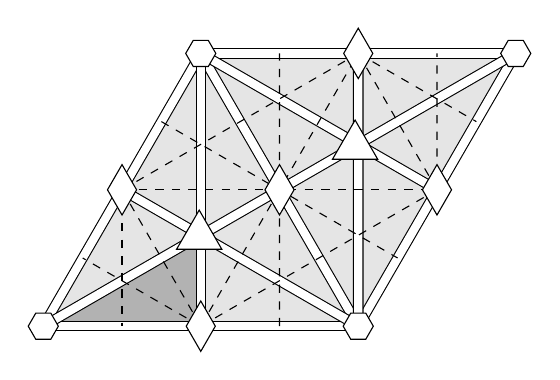
\begin{tikzpicture}
\coordinate (o) at (0,0);
\path (o) ++(0:\w) coordinate (a);
\path (o) ++(60:\w) coordinate (b);
\path (o) ++(30:{sqrt(3)*\w}) coordinate (c);
\coordinate (a1) at ($(o)!0.5!(a)$);    
\coordinate (a2) at ($(o)!0.25!(a)$);    
\coordinate (a3) at ($(o)!0.75!(a)$);    
\coordinate (b1) at ($(o)!0.5!(b)$);    
\coordinate (b2) at ($(o)!0.25!(b)$);    
\coordinate (b3) at ($(o)!0.75!(b)$);    
\coordinate (c1) at ($(o)!0.5!(c)$);    
\coordinate (c2) at ($(o)!0.33!(c)$);    
\coordinate (c3) at ($(o)!0.66!(c)$);    
\coordinate (d1) at ($(b)!0.5!(c)$);    
\coordinate (d2) at ($(b)!0.25!(c)$);    
\coordinate (d3) at ($(b)!0.75!(c)$);    
\coordinate (e1) at ($(a)!0.5!(c)$);    
\coordinate (e2) at ($(a)!0.25!(c)$);    
\coordinate (e3) at ($(a)!0.75!(c)$); 
\filldraw[black!10] (o)--(a)--(c)--(b)--cycle;   
\filldraw[black!30] (o)--(a1)--(c2)--cycle;   
\draw[double,double distance=3pt] (o) -- (a);
\draw[double,double distance=3pt] (a)-- (c);
\draw[double,double distance=3pt] (c)--(b);
\draw[double,double distance=3pt] (b) -- (o);

\draw[double,double distance=3pt] (o) -- (c);
\draw[double,double distance=3pt] (a) -- (b);

\draw[double,double distance=3pt] (a1) -- (b);
\draw[double,double distance=3pt] (a) -- (d1);

\draw[double,double distance=3pt] (b1) -- (a);
\draw[double,double distance=3pt] (b) -- (e1);

\draw[dashed] (a1)--(b2);
\draw[dashed] (a1)--(b1);
\draw[dashed] (a1)--(d1);
\draw[dashed] (a1)--(e1);
\draw[dashed] (b1)--(a2);
\draw[dashed] (b1)--(e1);
\draw[dashed] (b1)--(d1);
\draw[dashed] (d1)--(e1);
\draw[dashed] (d1)--(e3);
\draw[dashed] (e1)--(d3);
\draw[dashed] (a3)--(d2);
\draw[dashed] (b3)--(e2);

\foreach \h in {o,a,b,c}{
\node[shape aspect=1,regular polygon, regular polygon sides=6,draw=black,fill=white] at (\h) {};
}
\foreach \h in {a1,b1,c1,d1,e1}{
\node[shape aspect=1,kite,kite vertex angles=60,draw=black,fill=white] at (\h) {};
}
\foreach \h in {c2,c3}{
\node[shape aspect=1,regular polygon, regular polygon sides=3,draw=black,fill=white] at (\h) {};
}
\end{tikzpicture}
            \caption{p6m}
            \end{figure}
        \subsubsection{Has no reflection}
        \begin{figure}[H]
            \centering
            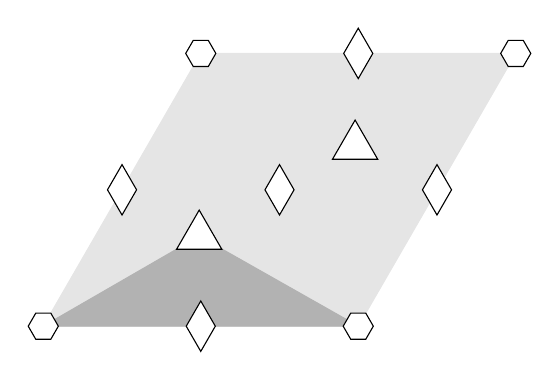
\begin{tikzpicture}
\coordinate (o) at (0,0);
\path (o) ++(0:\w) coordinate (a);
\path (o) ++(60:\w) coordinate (b);
\path (o) ++(30:{sqrt(3)*\w}) coordinate (c);
\coordinate (a1) at ($(o)!0.5!(a)$);    
\coordinate (a2) at ($(o)!0.25!(a)$);    
\coordinate (a3) at ($(o)!0.75!(a)$);    
\coordinate (b1) at ($(o)!0.5!(b)$);    
\coordinate (b2) at ($(o)!0.25!(b)$);    
\coordinate (b3) at ($(o)!0.75!(b)$);    
\coordinate (c1) at ($(o)!0.5!(c)$);    
\coordinate (c2) at ($(o)!0.33!(c)$);    
\coordinate (c3) at ($(o)!0.66!(c)$);    
\coordinate (d1) at ($(b)!0.5!(c)$);    
\coordinate (d2) at ($(b)!0.25!(c)$);    
\coordinate (d3) at ($(b)!0.75!(c)$);    
\coordinate (e1) at ($(a)!0.5!(c)$);    
\coordinate (e2) at ($(a)!0.25!(c)$);    
\coordinate (e3) at ($(a)!0.75!(c)$);
\filldraw[black!10] (o)--(a)--(c)--(b)--cycle;   
\filldraw[black!30] (o)--(a)--(c2)--cycle;   
\foreach \h in {o,a,b,c}{
\node[shape aspect=1,regular polygon, regular polygon sides=6,draw=black,fill=white] at (\h) {};
}
\foreach \h in {a1,b1,c1,d1,e1}{
\node[shape aspect=1,kite,kite vertex angles=60,draw=black,fill=white] at (\h) {};
}
\foreach \h in {c2,c3}{
\node[shape aspect=1,regular polygon, regular polygon sides=3,draw=black,fill=white] at (\h) {};
}
\end{tikzpicture}
            \caption{p6}
        \end{figure}
    \end{multicols}
    \subsection{\ang{90} rotational summetry}
    \begin{multicols}{2}
        \subsubsection{Has reflection with mirrors at \ang{45}}
        \begin{figure}[H]
            \centering
            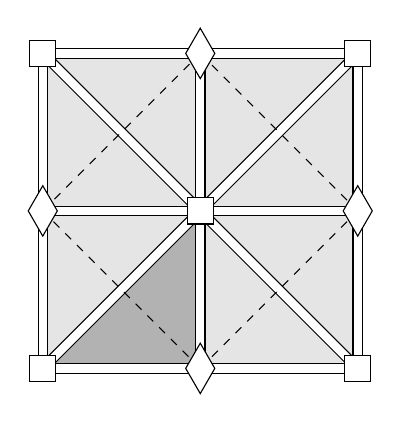
\begin{tikzpicture}
\coordinate (o) at (0,0);
\path (o) ++(0:\w) coordinate (a);
\path (o) ++(90:\w) coordinate (b);
\path (o) ++(45:{sqrt(2)*\w}) coordinate (c);
\coordinate (a1) at ($(o)!0.5!(a)$);    
\coordinate (b1) at ($(o)!0.5!(b)$);    
\coordinate (c1) at ($(o)!0.5!(c)$);    
\coordinate (d1) at ($(b)!0.5!(c)$);    
\coordinate (e1) at ($(a)!0.5!(c)$);    
\filldraw[black!10] (o)--(a)--(c)--(b)--cycle;   
\filldraw[black!30] (o)--(a1)--(c1)--cycle;   
\draw[double,double distance=3pt] (o) -- (a);
\draw[double,double distance=3pt] (a)-- (c);
\draw[double,double distance=3pt] (c)--(b);
\draw[double,double distance=3pt] (b) -- (o);

\draw[double,double distance=3pt] (o) -- (c);
\draw[double,double distance=3pt] (a) -- (b);

\draw[double,double distance=3pt] (a1) -- (d1);
\draw[double,double distance=3pt] (b1) -- (e1);

\draw[dashed] (a1)--(b1);
\draw[dashed] (a1)--(e1);
\draw[dashed] (b1)--(d1);
\draw[dashed] (d1)--(e1);
\foreach \h in {o,a,b,c,c1}{
\node[shape aspect=1,regular polygon, regular polygon sides=4,draw=black,fill=white] at (\h) {};
}
\foreach \h in {a1,b1,d1,e1}{
\node[shape aspect=1,kite,kite vertex angles=60,draw=black,fill=white] at (\h) {};
}
\end{tikzpicture}
            \caption{p4m}
        \end{figure}
        \subsubsection{It Has reflection but no mirrors at \ang{45}}
            \begin{figure}[H]
                \centering
                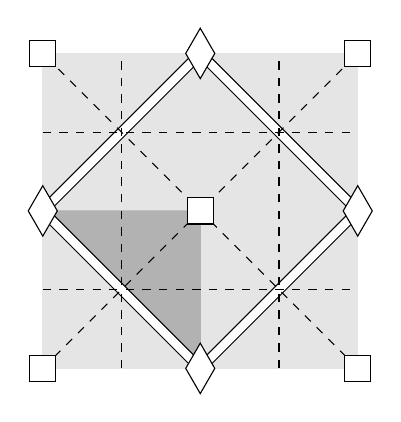
\begin{tikzpicture}
\coordinate (o) at (0,0);
\path (o) ++(0:\w) coordinate (a);
\path (o) ++(90:\w) coordinate (b);
\path (o) ++(45:{sqrt(2)*\w}) coordinate (c);
\coordinate (a1) at ($(o)!0.5!(a)$);
\coordinate (a2) at ($(o)!0.25!(a)$);    
\coordinate (a3) at ($(o)!0.75!(a)$);    

\coordinate (b1) at ($(o)!0.5!(b)$);   
\coordinate (b2) at ($(o)!0.25!(b)$);     
\coordinate (b3) at ($(o)!0.75!(b)$);     
\coordinate (c1) at ($(o)!0.5!(c)$);    
\coordinate (d1) at ($(b)!0.5!(c)$);    
\coordinate (d2) at ($(b)!0.25!(c)$);    
\coordinate (d3) at ($(b)!0.75!(c)$);    
\coordinate (e1) at ($(a)!0.5!(c)$);    
\coordinate (e2) at ($(a)!0.25!(c)$);    
\coordinate (e3) at ($(a)!0.75!(c)$); 
\filldraw[black!10] (o)--(a)--(c)--(b)--cycle;   
\filldraw[black!30] (a1)--(c1)--(b1)--cycle;   

\draw[double,double distance=3pt] (a1) -- (b1);
\draw[double,double distance=3pt] (b1) -- (d1);
\draw[double,double distance=3pt] (d1) -- (e1);
\draw[double,double distance=3pt] (e1) -- (a1);

\draw[dashed] (o)--(c);
\draw[dashed] (a)--(b);
\draw[dashed] (a2)--(d2);
\draw[dashed] (a3)--(d3);
\draw[dashed] (b2)--(e2);
\draw[dashed] (b3)--(e3);
\foreach \h in {o,a,b,c,c1}{
\node[shape aspect=1,regular polygon, regular polygon sides=4,draw=black,fill=white] at (\h) {};
}
\foreach \h in {a1,b1,d1,e1}{
\node[shape aspect=1,kite,kite vertex angles=60,draw=black,fill=white] at (\h) {};
}
\end{tikzpicture}
                \caption{p4g}
            \end{figure}
        \end{multicols}
        \subsubsection{No reflection}
        \begin{figure}[H]
                    \centering
                    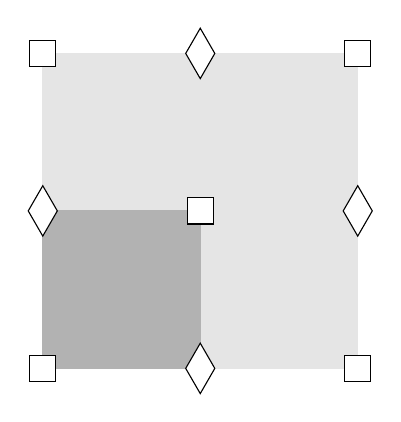
\begin{tikzpicture}
                    \coordinate (o) at (0,0);
                    \path (o) ++(0:\w) coordinate (a);
                    \path (o) ++(90:\w) coordinate (b);
                    \path (o) ++(45:{sqrt(2)*\w}) coordinate (c);
                    \coordinate (a1) at ($(o)!0.5!(a)$);
                    \coordinate (a2) at ($(o)!0.25!(a)$);    
                    \coordinate (a3) at ($(o)!0.75!(a)$);    
    
                    \coordinate (b1) at ($(o)!0.5!(b)$);   
                    \coordinate (b2) at ($(o)!0.25!(b)$);     
                    \coordinate (b3) at ($(o)!0.75!(b)$);     
                    \coordinate (c1) at ($(o)!0.5!(c)$);    
                    \coordinate (d1) at ($(b)!0.5!(c)$);    
                    \coordinate (d2) at ($(b)!0.25!(c)$);    
                    \coordinate (d3) at ($(b)!0.75!(c)$);    
                    \coordinate (e1) at ($(a)!0.5!(c)$);    
                    \coordinate (e2) at ($(a)!0.25!(c)$);    
                    \coordinate (e3) at ($(a)!0.75!(c)$); 
                    \filldraw[black!10] (o)--(a)--(c)--(b)--cycle;   
                    \filldraw[black!30] (o)--(a1)--(c1)--(b1)--cycle;   
                    \foreach \h in {o,a,b,c,c1}{
                    \node[shape aspect=1,regular polygon, regular polygon sides=4,draw=black,fill=white] at (\h) {};
                    }
                    \foreach \h in {a1,b1,d1,e1}{
                    \node[shape aspect=1,kite,kite vertex angles=60,draw=black,fill=white] at (\h) {};
                    }
                    \end{tikzpicture}
                    \caption{p4}
                \end{figure}
    \subsection{\ang{120} rotational summetry}
        \subsubsection{Has no reflection}
        \begin{figure}[H]
                    \centering
                    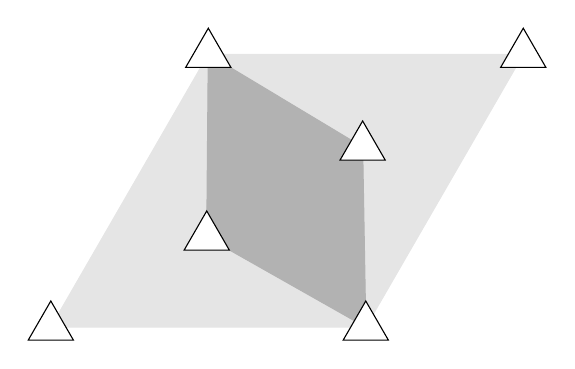
\begin{tikzpicture}
                    \coordinate (o) at (0,0);
                    \path (o) ++(0:\w) coordinate (a);
                    \path (o) ++(60:\w) coordinate (b);
                    \path (o) ++(30:{sqrt(3)*\w}) coordinate (c);
                    \coordinate (c2) at ($(o)!0.33!(c)$);    
                    \coordinate (c3) at ($(o)!0.66!(c)$);    
                    \filldraw[black!10] (o)--(a)--(c)--(b)--cycle;   
                    \filldraw[black!30] (a)--(c2)--(b)--(c3)--cycle;
                    \foreach \h in {o,a,b,c,c2,c3}{
                    \node[shape aspect=1,regular polygon, regular polygon sides=3,draw=black,fill=white] at (\h) {};
                    }
                    \end{tikzpicture}
                    \caption{p3}
                \end{figure}
        \begin{multicols}{2}
        \subsubsection{Has rotocenter off mirrors}
                \begin{figure}[H]
                    \centering
                    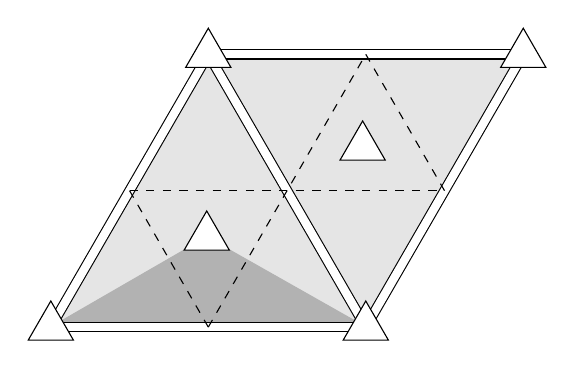
\begin{tikzpicture}
                    \coordinate (o) at (0,0);
                    \path (o) ++(0:\w) coordinate (a);
                    \path (o) ++(60:\w) coordinate (b);
                    \path (o) ++(30:{sqrt(3)*\w}) coordinate (c);
                    \coordinate (a1) at ($(o)!0.5!(a)$);    
                    \coordinate (b1) at ($(o)!0.5!(b)$);    
                    \coordinate (c2) at ($(o)!0.33!(c)$);    
                    \coordinate (c3) at ($(o)!0.66!(c)$);    
                    \coordinate (d1) at ($(b)!0.5!(c)$);    
                    \coordinate (e1) at ($(a)!0.5!(c)$);    
                    \filldraw[black!10] (o)--(a)--(c)--(b)--cycle;   
                    \filldraw[black!30] (o)--(a)--(c2)--cycle;   
                    \draw[double,double distance=3pt] (o) -- (a);
                    \draw[double,double distance=3pt] (a)-- (c);
                    \draw[double,double distance=3pt] (c)--(b);
                    \draw[double,double distance=3pt] (b) -- (o);
                    \draw[double,double distance=3pt] (a) -- (b);
                    \draw[dashed] (a1)--(b1);
                    \draw[dashed] (a1)--(d1);
                    \draw[dashed] (b1)--(e1);
                    \draw[dashed] (d1)--(e1);
                    \foreach \h in {o,a,b,c,c2,c3}{
                    \node[shape aspect=1,regular polygon, regular polygon sides=3,draw=black,fill=white] at (\h) {};
                    }
                    \end{tikzpicture}
                    \caption{p31m}
                \end{figure}        
        \subsubsection{Has rotocenter along mirrors}
                \begin{figure}[H]
                    \centering
                    \include{p3m1}
                    \caption{p3m1}
                \end{figure}  
            \end{multicols} 
    \subsection{\ang{180} rotational summetry}
            \begin{multicols}{2}
        \subsubsection{Has no glide reflection}
        \begin{figure}[H]
                    \centering
                    \include{p2}
                    \caption{p2}
                \end{figure}
        \subsubsection{Has glide reflection}
        \begin{figure}[H]
                    \centering
                    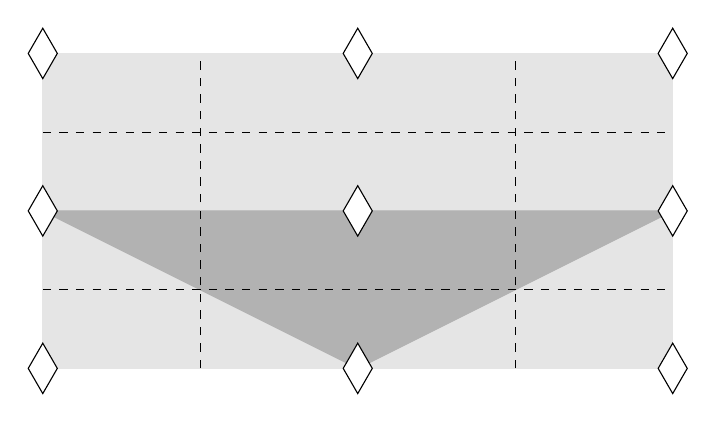
\begin{tikzpicture}
                    \coordinate (o) at (0,0);
                    \path (o) ++(0:2*\w) coordinate (a);
                    \path (o) ++(90:\w) coordinate (b);
                    \path (a) ++(90:{\w}) coordinate (c);
                    \coordinate (a1) at ($(o)!0.5!(a)$);
                    \coordinate (a1) at ($(o)!0.5!(a)$);    
                    \coordinate (a2) at ($(o)!0.25!(a)$);    
                    \coordinate (a3) at ($(o)!0.75!(a)$);    
                    \coordinate (b1) at ($(o)!0.5!(b)$);    
                    \coordinate (b2) at ($(o)!0.25!(b)$);    
                    \coordinate (b3) at ($(o)!0.75!(b)$);    
                    \coordinate (c1) at ($(o)!0.5!(c)$);    
                    \coordinate (d1) at ($(b)!0.5!(c)$);    
                    \coordinate (d2) at ($(b)!0.25!(c)$);    
                    \coordinate (d3) at ($(b)!0.75!(c)$);    
                    \coordinate (e1) at ($(a)!0.5!(c)$);    
                    \coordinate (e2) at ($(a)!0.25!(c)$);    
                    \coordinate (e3) at ($(a)!0.75!(c)$);    
                    \filldraw[black!10] (o)--(a)--(c)--(b)--cycle;   
                    \filldraw[black!30] (a1)--(b1)--(e1)--cycle;   
                    \draw[dashed] (a2)--(d2);
                    \draw[dashed] (b2)--(e2);
                    \draw[dashed] (a3)--(d3);
                    \draw[dashed] (b3)--(e3);
                    \foreach \h in {o,a,b,c,a1,b1,c1,d1,e1}{
                    \node[shape aspect=1,kite,kite vertex angles=60,draw=black,fill=white] at (\h) {};
                    }
                    \end{tikzpicture}
                    \caption{pgg}
                \end{figure}
            \end{multicols}
        \subsubsection{Has no perpendicular reflection}
            \begin{figure}[H]
                    \centering
                    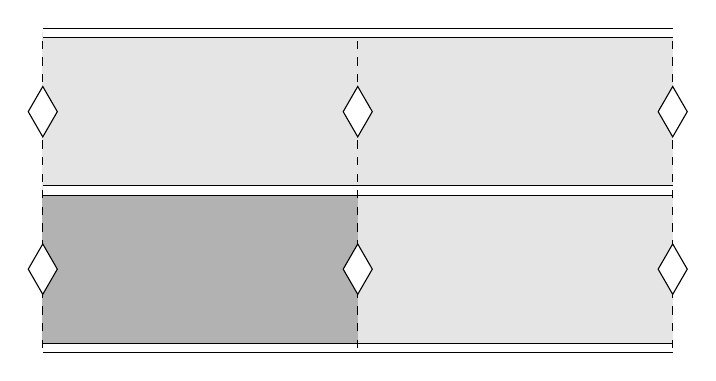
\begin{tikzpicture}
\coordinate (o) at (0,0);
\path (o) ++(0:2*\w) coordinate (a);
\path (o) ++(90:\w) coordinate (b);
\path (a) ++(90:{\w}) coordinate (c);
\coordinate (a1) at ($(o)!0.5!(a)$);     
\coordinate (b1) at ($(o)!0.5!(b)$);    
\coordinate (b2) at ($(o)!0.25!(b)$);    
\coordinate (b3) at ($(o)!0.75!(b)$);    
\coordinate (c1) at ($(o)!0.5!(c)$);    
\coordinate (d1) at ($(b)!0.5!(c)$);     
\coordinate (e1) at ($(a)!0.5!(c)$);    
\coordinate (e2) at ($(a)!0.25!(c)$);    
\coordinate (e3) at ($(a)!0.75!(c)$);    
\coordinate (f2) at ($(a1)!0.25!(d1)$);    
\coordinate (f3) at ($(a1)!0.75!(d1)$);    
\filldraw[black!10] (o)--(a)--(c)--(b)--cycle;   
\filldraw[black!30] (o)--(a1)--(c1)--(b1)--cycle;   
\draw[double,double distance=3pt] (o) -- (a);
\draw[double,double distance=3pt] (b) -- (c);
\draw[double,double distance=3pt] (b1) -- (e1);
\draw[dashed] (a1)--(d1);
\draw[dashed] (o)--(b);
\draw[dashed] (a)--(c);
\foreach \h in {b2,b3,e2,e3,f2,f3}{
\node[shape aspect=1,kite,kite vertex angles=60,draw=black,fill=white] at (\h) {};
}
\end{tikzpicture}
                    \caption{pmg}
                \end{figure}
                    \begin{multicols}{2}
        \subsection{Has perpendicular reflection with rotocenter off mirrors}
        \begin{figure}[H]
                    \centering
                    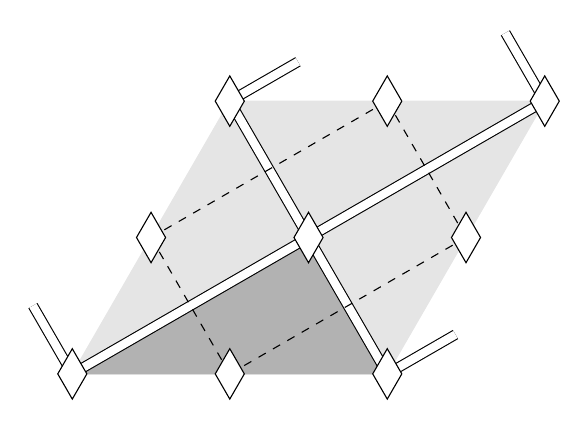
\begin{tikzpicture}
\coordinate (o) at (0,0);
\path (o) ++(0:\w) coordinate (a);
\path (o) ++(60:\w) coordinate (b);
\path (o) ++(30:{sqrt(3)*\w}) coordinate (c);
\coordinate (a1) at ($(o)!0.5!(a)$);     
\coordinate (b1) at ($(o)!0.5!(b)$);    
\coordinate (c1) at ($(o)!0.5!(c)$);    
\coordinate (d1) at ($(b)!0.5!(c)$);     
\coordinate (e1) at ($(a)!0.5!(c)$);    
\coordinate (e2) at ($(a)!0.25!(c)$);    
\coordinate (e3) at ($(a)!0.75!(c)$);    
\filldraw[black!10] (o)--(a)--(c)--(b)--cycle;   
\filldraw[black!30] (o)--(a)--(c1)--cycle;   
\draw[double,double distance=3pt] (o) -- (c);
\draw[double,double distance=3pt] (b) -- (a);
\draw[double,double distance=3pt] (a) --++ (30:1);
\draw[double,double distance=3pt] (b) --++ (30:1);
\draw[double,double distance=3pt] (o) --++ (120:1);
\draw[double,double distance=3pt] (c) --++ (120:1);

\draw[dashed] (a1)--(e1);
\draw[dashed] (b1)--(a1);
\draw[dashed] (d1)--(b1);
\draw[dashed] (e1)--(d1);
\foreach \h in {o,a,b,c,a1,b1,c1,d1,e1}{
\node[shape aspect=1,kite,kite vertex angles=60,draw=black,fill=white] at (\h) {};
}
\end{tikzpicture}
                    \caption{cmm}
                    \end{figure} 
        \subsection{Has perpendicular reflection with rotocenter along mirrors}
        \begin{figure}[H]
                    \centering
                    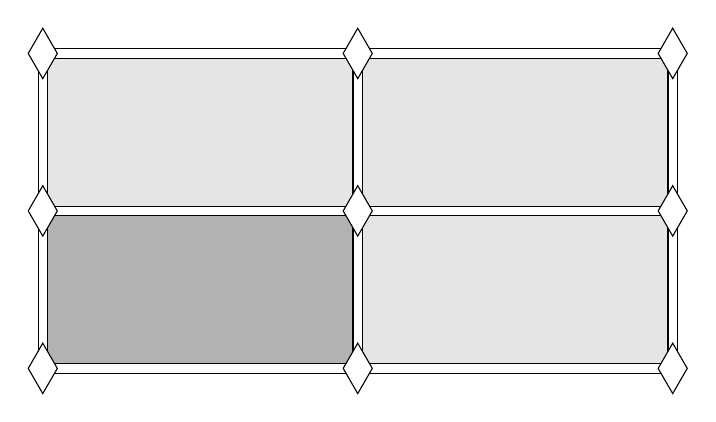
\begin{tikzpicture}
\coordinate (o) at (0,0);
\path (o) ++(0:2*\w) coordinate (a);
\path (o) ++(90:\w) coordinate (b);
\path (a) ++(90:{\w}) coordinate (c);
\coordinate (a1) at ($(o)!0.5!(a)$);     
\coordinate (b1) at ($(o)!0.5!(b)$);    
\coordinate (c1) at ($(o)!0.5!(c)$);    
\coordinate (d1) at ($(b)!0.5!(c)$);     
\coordinate (e1) at ($(a)!0.5!(c)$);    
\filldraw[black!10] (o)--(a)--(c)--(b)--cycle;   
\filldraw[black!30] (o)--(a1)--(c1)--(b1)--cycle;   
\draw[double,double distance=3pt] (o) -- (a);
\draw[double,double distance=3pt] (a) -- (c);
\draw[double,double distance=3pt] (b) -- (c);
\draw[double,double distance=3pt] (b) -- (o);
\draw[double,double distance=3pt] (b1) -- (e1);
\draw[double,double distance=3pt] (a1) -- (d1);
\foreach \h in {o,a,b,c,a1,b1,c1,d1,e1}{
\node[shape aspect=1,kite,kite vertex angles=60,draw=black,fill=white] at (\h) {};
}
\end{tikzpicture}
                    \caption{pmm}
                    \end{figure}
                \end{multicols}
\section{Has no rotational symmetry}
                    \begin{multicols}{2}
\subsection{Has no glide reflection}
\begin{figure}[H]
            \centering
            
\begin{tikzpicture}
\coordinate (o) at (0,0);
\path (o) ++(0:\w) coordinate (a);
\path (o) ++(60:\w) coordinate (b);
\path (o) ++(30:{sqrt(3)*\w}) coordinate (c);
\filldraw[black!30] (o)--(a)--(c)--(b)--cycle;   
\end{tikzpicture}
            \caption{p1}
            \end{figure}

            \subsection{Has glide reflection}
            \begin{figure}[H]
            \centering
            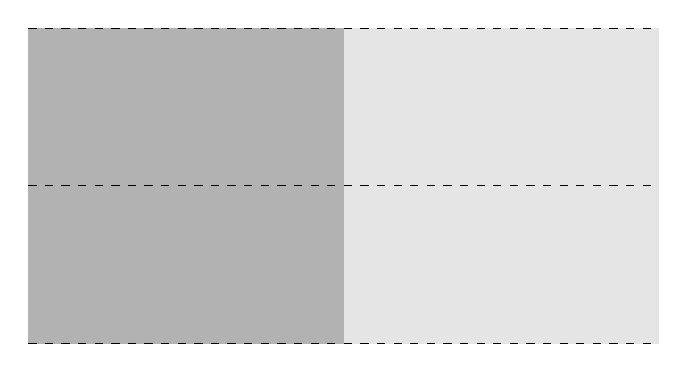
\begin{tikzpicture}
\coordinate (o) at (0,0);
\path (o) ++(0:2*\w) coordinate (a);
\path (o) ++(90:\w) coordinate (b);
\path (a) ++(90:{\w}) coordinate (c);
\coordinate (a1) at ($(o)!0.5!(a)$);    
\coordinate (b1) at ($(o)!0.5!(b)$);    
\coordinate (d1) at ($(b)!0.5!(c)$);    
\coordinate (e1) at ($(a)!0.5!(c)$);    
\filldraw[black!10] (o)--(a)--(c)--(b)--cycle;   
\filldraw[black!30] (o)--(a1)--(d1)--(b)--cycle;   
\draw[dashed] (o) -- (a);
\draw[dashed] (b) -- (c);
\draw[dashed] (b1) -- (e1);
\end{tikzpicture}
            \caption{pg}
            \end{figure}
        \end{multicols}
        \newpage
\begin{multicols}{2}

            \subsection{Has glide axis off mirrors}
            \begin{figure}[H]
            \centering
            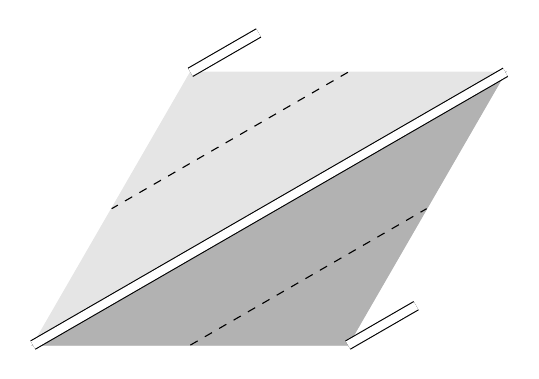
\begin{tikzpicture}
\coordinate (o) at (0,0);
\path (o) ++(0:\w) coordinate (a);
\path (o) ++(60:\w) coordinate (b);
\path (o) ++(30:{sqrt(3)*\w}) coordinate (c);
\coordinate (a1) at ($(o)!0.5!(a)$);     
\coordinate (b1) at ($(o)!0.5!(b)$);    
\coordinate (c1) at ($(o)!0.5!(c)$);    
\coordinate (d1) at ($(b)!0.5!(c)$);     
\coordinate (e1) at ($(a)!0.5!(c)$);    
\filldraw[black!10] (o)--(a)--(c)--(b)--cycle;   
\filldraw[black!30] (o)--(a)--(c)--cycle;   
\draw[double,double distance=3pt] (o) -- (c);
\draw[double,double distance=3pt] (a) --++ (30:1);
\draw[double,double distance=3pt] (b) --++ (30:1);
\draw[dashed] (a1)--(e1);
\draw[dashed] (d1)--(b1);
\end{tikzpicture}
            \caption{cm}
            \end{figure}
            \subsection{Has glide axis along mirrors}
            \begin{figure}[H]
            \centering
            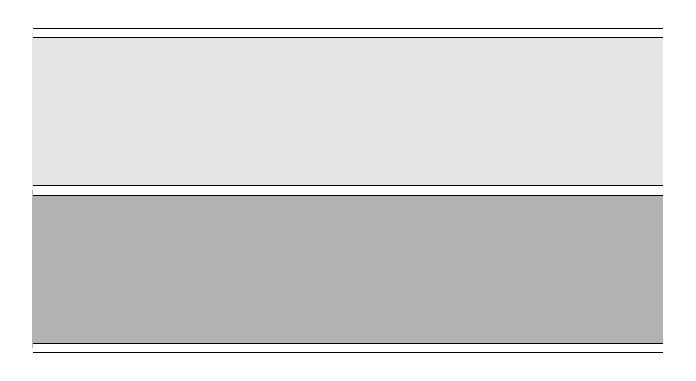
\begin{tikzpicture}
\coordinate (o) at (0,0);
\path (o) ++(0:2*\w) coordinate (a);
\path (o) ++(90:\w) coordinate (b);
\path (a) ++(90:{\w}) coordinate (c);
\coordinate (b1) at ($(o)!0.5!(b)$);    
\coordinate (e1) at ($(a)!0.5!(c)$);    
\filldraw[black!10] (o)--(a)--(c)--(b)--cycle;   
\filldraw[black!30] (o)--(a)--(e1)--(b1)--cycle;   
\draw[double,double distance=3pt] (o) -- (a);
\draw[double,double distance=3pt] (b) -- (c);
\draw[double,double distance=3pt] (b1) -- (e1);
\end{tikzpicture}
            \caption{pm}
            \end{figure}
        \end{multicols}

\vfill
This document was prepared for Maths is Fun: symmetry program on 1 Feb 2026 at SGB by Disha Kuzhively, not for circulation.
\end{document}
\usepackage[inkscapearea=page]{svg}

\usepackage{adjustbox}
